\documentclass[a4paper,14pt]{extarticle}
\usepackage[utf8]{inputenc}
\usepackage[T1]{fontenc}
\usepackage[russian]{babel}
\usepackage{indentfirst}
\usepackage{geometry}
\usepackage{fontspec}
\usepackage{wrapfig}
\usepackage[explicit]{titlesec}
\usepackage{longtable}
\usepackage{graphicx}
\usepackage{float}
\usepackage{array}
\usepackage[
    figurename=Рисунок,
    labelsep=endash,
]{caption}
\usepackage{hyperref}
\usepackage{tocloft}

\geometry{
    left=30mm,
    top=20mm,
    bottom=20mm,
    right=15mm,
}

\setmainfont{Times New Roman}

\hypersetup{
    colorlinks=true,
    linkcolor=black,
}

\titleformat{\section}
{\normalfont}{\bfseries \thesection.}{4pt}{\bfseries #1}

\titleformat{\subsection}
{\normalfont}{\bfseries \thesubsection.}{4pt}{\bfseries #1}

\renewcommand{\baselinestretch}{1.5}

\captionsetup{width=\textwidth}
\captionsetup[table]{singlelinecheck=off,justification=raggedright}

\renewcommand{\cftsecleader}{\cftdotfill{\cftdotsep}}
\renewcommand{\cftsecaftersnum}{.}%

\addto\captionsrussian{\renewcommand{\contentsname}{Содержание\hfill}}
\renewcommand{\cfttoctitlefont}{\hfill\bfseries}
\renewcommand{\cftaftertoctitle}{\hfill}

\setlength\LTcapwidth{\textwidth}
\setlength\LTleft{0pt}
\setlength\LTright{0pt}

\begin{document}

\begin{titlepage}
    \vspace{0pt plus2fill}
    \noindent

    \vspace{0pt plus6fill}
    \begin{center}
        Министерство образования и науки

        федеральное государственное автономное образовательное учреждение высшего образования

        <<Национальный исследовательский университет ИТМО>>

        Факультет инфокоммуникационных технологий

        \vspace{0pt plus8fill}

        Отчет по курсу: \textbf{<<Базы данных>>}

        \textbf{<<Интернет площадка креативных товаров>>}
    \end{center}

    \vspace{0pt plus8fill}
    \begin{flushright}
        Выполнили: \\
        Швалов Даниил Андреевич \\
        Осыченко Арсений Дмитриевич \\
        Богданов Михаил Александрович \\
        Ларичева Дарья Кирилловна \\
        Карагодин Максим Александрович

        Группа: К32211

        Проверила: \\
        Осетрова Ирина Станиславовна
    \end{flushright}

    \vspace{0pt plus5fill}
    \begin{center}
        Санкт-Петербург \\ 2022
    \end{center}
\end{titlepage}

\setcounter{page}{2}

\tableofcontents
\newpage

\section{Введение}

Уже достаточно долгое время интернет-площадки для покупки и продажи вещей пользуются огромной популярностью. На рынке существует множество площадок, предоставляющих сервис для продажи различных видов товаров.

<<Креатистор>> -- это интернет-площадка для креативных людей, интересных идей и уникальных товаров. На рынке существует множество различных магазинов креативных товаров. Однако мы готовы предложить сервис, отличный от существующих.

Мы, равно как наши конкуренты, не покупаем и не продаем товары. Наша компания предоставляем площадку, на которой продавцы находят своих покупателей, а покупатели получают возможность приобрести креативные товары. Однако, в отличии от остальных площадок мы ориентированы не на масс-маркет, а на нишу людей, интересующимся креативными вещами.

\section{Цели}

Целью данной лабораторной работы является разработка логической схемы базы данных для интернет-площадки по продаже креативных вещей.

\section{Задачи}

Для достижения поставленной цели необходимо выполнить следующие задачи:
\begin{itemize}
    \item анализ предметной области;
    % \item анализ существующих аналогов;
    \item анализ пользовательских возможностей;
    \item выделение основных сущностей;
    \item определение связей между сущностями;
    \item создание UML-модели.
\end{itemize}

\section{Концепт интернет-площадки}

Интернет площадка <<Креатистор>> достаточно сильно похожа на существующие аналоги. Это не удивительно, поскольку достаточно сложно придумать что-то новое в хорошо освоенной сфере. Однако у нашей площадки есть некоторые особенности, которые отличают нас от остальных. Основная особенность заключается в том, что наша площадка ориентирована на креативных людей, предлагающих креативные товары.

Разберем эту идею подробнее, а точнее, каким образом мы собираемся ее реализовать. В первую очередь рассмотрим то, каким способом мы собираемся оставаться площадкой с креативными товарами. Наш способ -- модерация. Именно модерация -- это первое, что отличает по части реализации нашу платформу от своих аналогов. Поскольку наша площадка стремится быть местом только с креативными товарами, нам необходимо проверять каждое объявление. Это позволит избежать продажи некачественного товара, а также товаров широкого потребления.

Еще одно отличие -- это поддержания почти полного равноправия на площадке. Во многих сервисах по продаже товаров предусмотрены способы по продвижению своих товаров. Так, например, это может быть поднятие объявления в поиске или закрепление его. На нашей площадке этого не предусмотрено. Мы считаем, что объявления должны выдаваться только в порядке качества заполнения информации о товаре: чем подробнее, точнее и качественнее написано описание товара, тем более вероятно, что именно этот товар попадется в поиске. В то же время, благодаря модерации будут исключены случаи подкрутки описания под поисковые алгоритмы.

Однако тут же возникает вопрос о монетизации платформы. Именно из-за монетизации на нашей платформе только почти равноправие. Особенностью нашей платформы является то, что только пользователи с подпиской могут добавлять свои товары. Другими словами, чтобы добавить свой товар на нашу платформу, пользователю необходимо приобрести подписки. Однако это никак не распространяется на просмотр и поиск объявлений: даже незарегистрированный пользователь может искать и просматривать объявления на нашей платформе.

Итого, наша платформа имеет следующие аспекты, отличающие нас от наших конкурентов:
\begin{itemize}
    \item модерация товаров;
    \item отсутствие методов продвижения товаров;
    \item подписочная система.
\end{itemize}

% \section{Анализ существующих аналогов}

% \subsection{Авито}

% \subsection{Юла}

% \subsection{Фарпост}

\section{Пользовательские возможности}

В этом разделе описан основной функционал, предоставленный пользователю. При взаимодействии с площадкой пользователь может:
\begin{itemize}
    \item создавать, входить в личный аккаунт;
    \item просматривать и искать товары;
    \item приобретать подписку, расширяющую доступный функционал;
    \item создавать и редактировать товары;
    \item добавлять товары в избранное;
    \item оставлять отзывы на продавцов;
    \item общаться с продавцом с помощью чата.
\end{itemize}
Рассмотрим каждый функционал поподробнее.

\subsection{Просмотр и поиск товаров}

Первое, с чем будет взаимодействовать пользователь -- это товары, который он присматривает себе. Кроме привычной ленты товаров, наша платформа предлагает поиск по товарам. На нем сделан особый акцент, потому что он несколько отличается от привычного поиска на торговых площадках.

\begin{figure}[H]
    \centering
    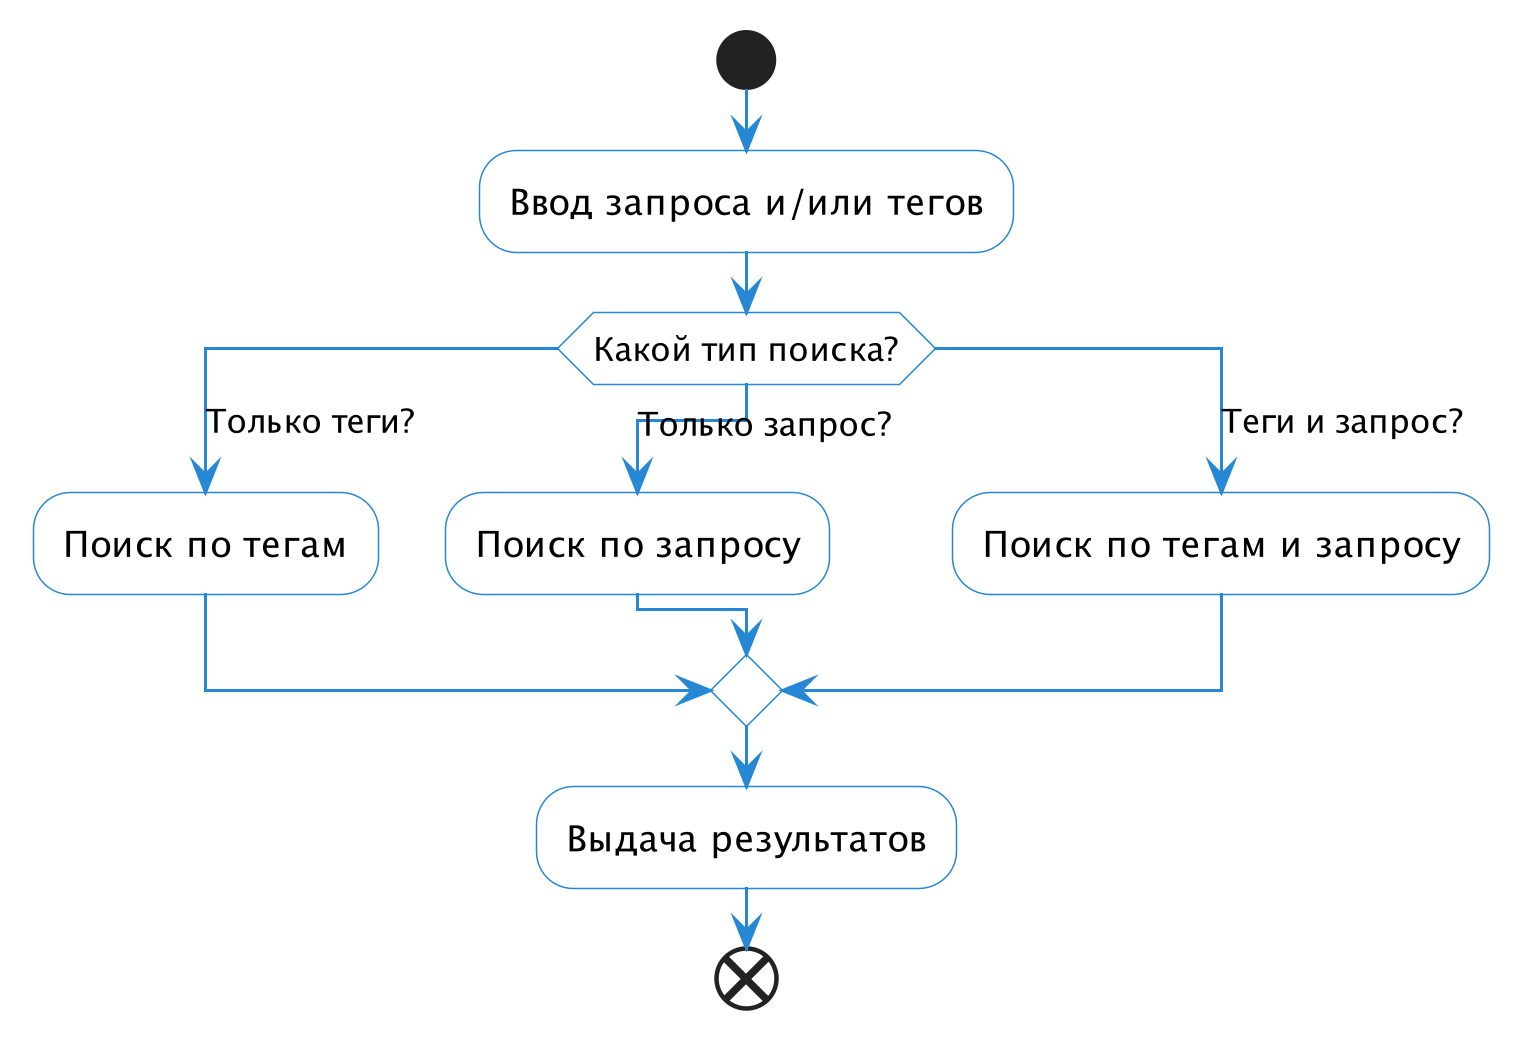
\includegraphics[width=0.8\textwidth]{images/search.png}
    \caption{Диаграмма поиска товаров}
\end{figure}

Как говорилось ранее, наша площадка рассчитана на креативные товары, а потому какие-то конкретные категории выделить очень сложно. Именно поэтому вместо категорий на нашей площадке используются теги. Эти теги похожи на привычные теги из социальных сетей: добавляет их продавец, а нужны они для упрощения поиска. Кроме тегов, также можно использовать обычный текстовый поиск.

\subsection{Взаимодействие с товарами}

Основной функционал нашей площадки завязан на товарах. В этом разделе будет рассмотрены следующие возможности по взаимодействию с товарами:
\begin{itemize}
    \item выставление товара на продажу;
    \item изменение товара;
    \item добавление товара в избранное.
\end{itemize}

\subsubsection*{Выставление товара на продажу}

Рассмотрим подробнее процесс выставления товару на продажу. Для этого зарегистрированный пользователь с подпиской должен заполнить форму, в которой он должен добавить следующую информацию о товаре:
\begin{itemize}
    \item название товара;
    \item стоимость;
    \item описание;
    \item изображения товара.
\end{itemize}
Кроме того, пользователь может добавить свои контактные данные в виде телефона и адреса электронной почты.

\begin{figure}[H]
    \centering
    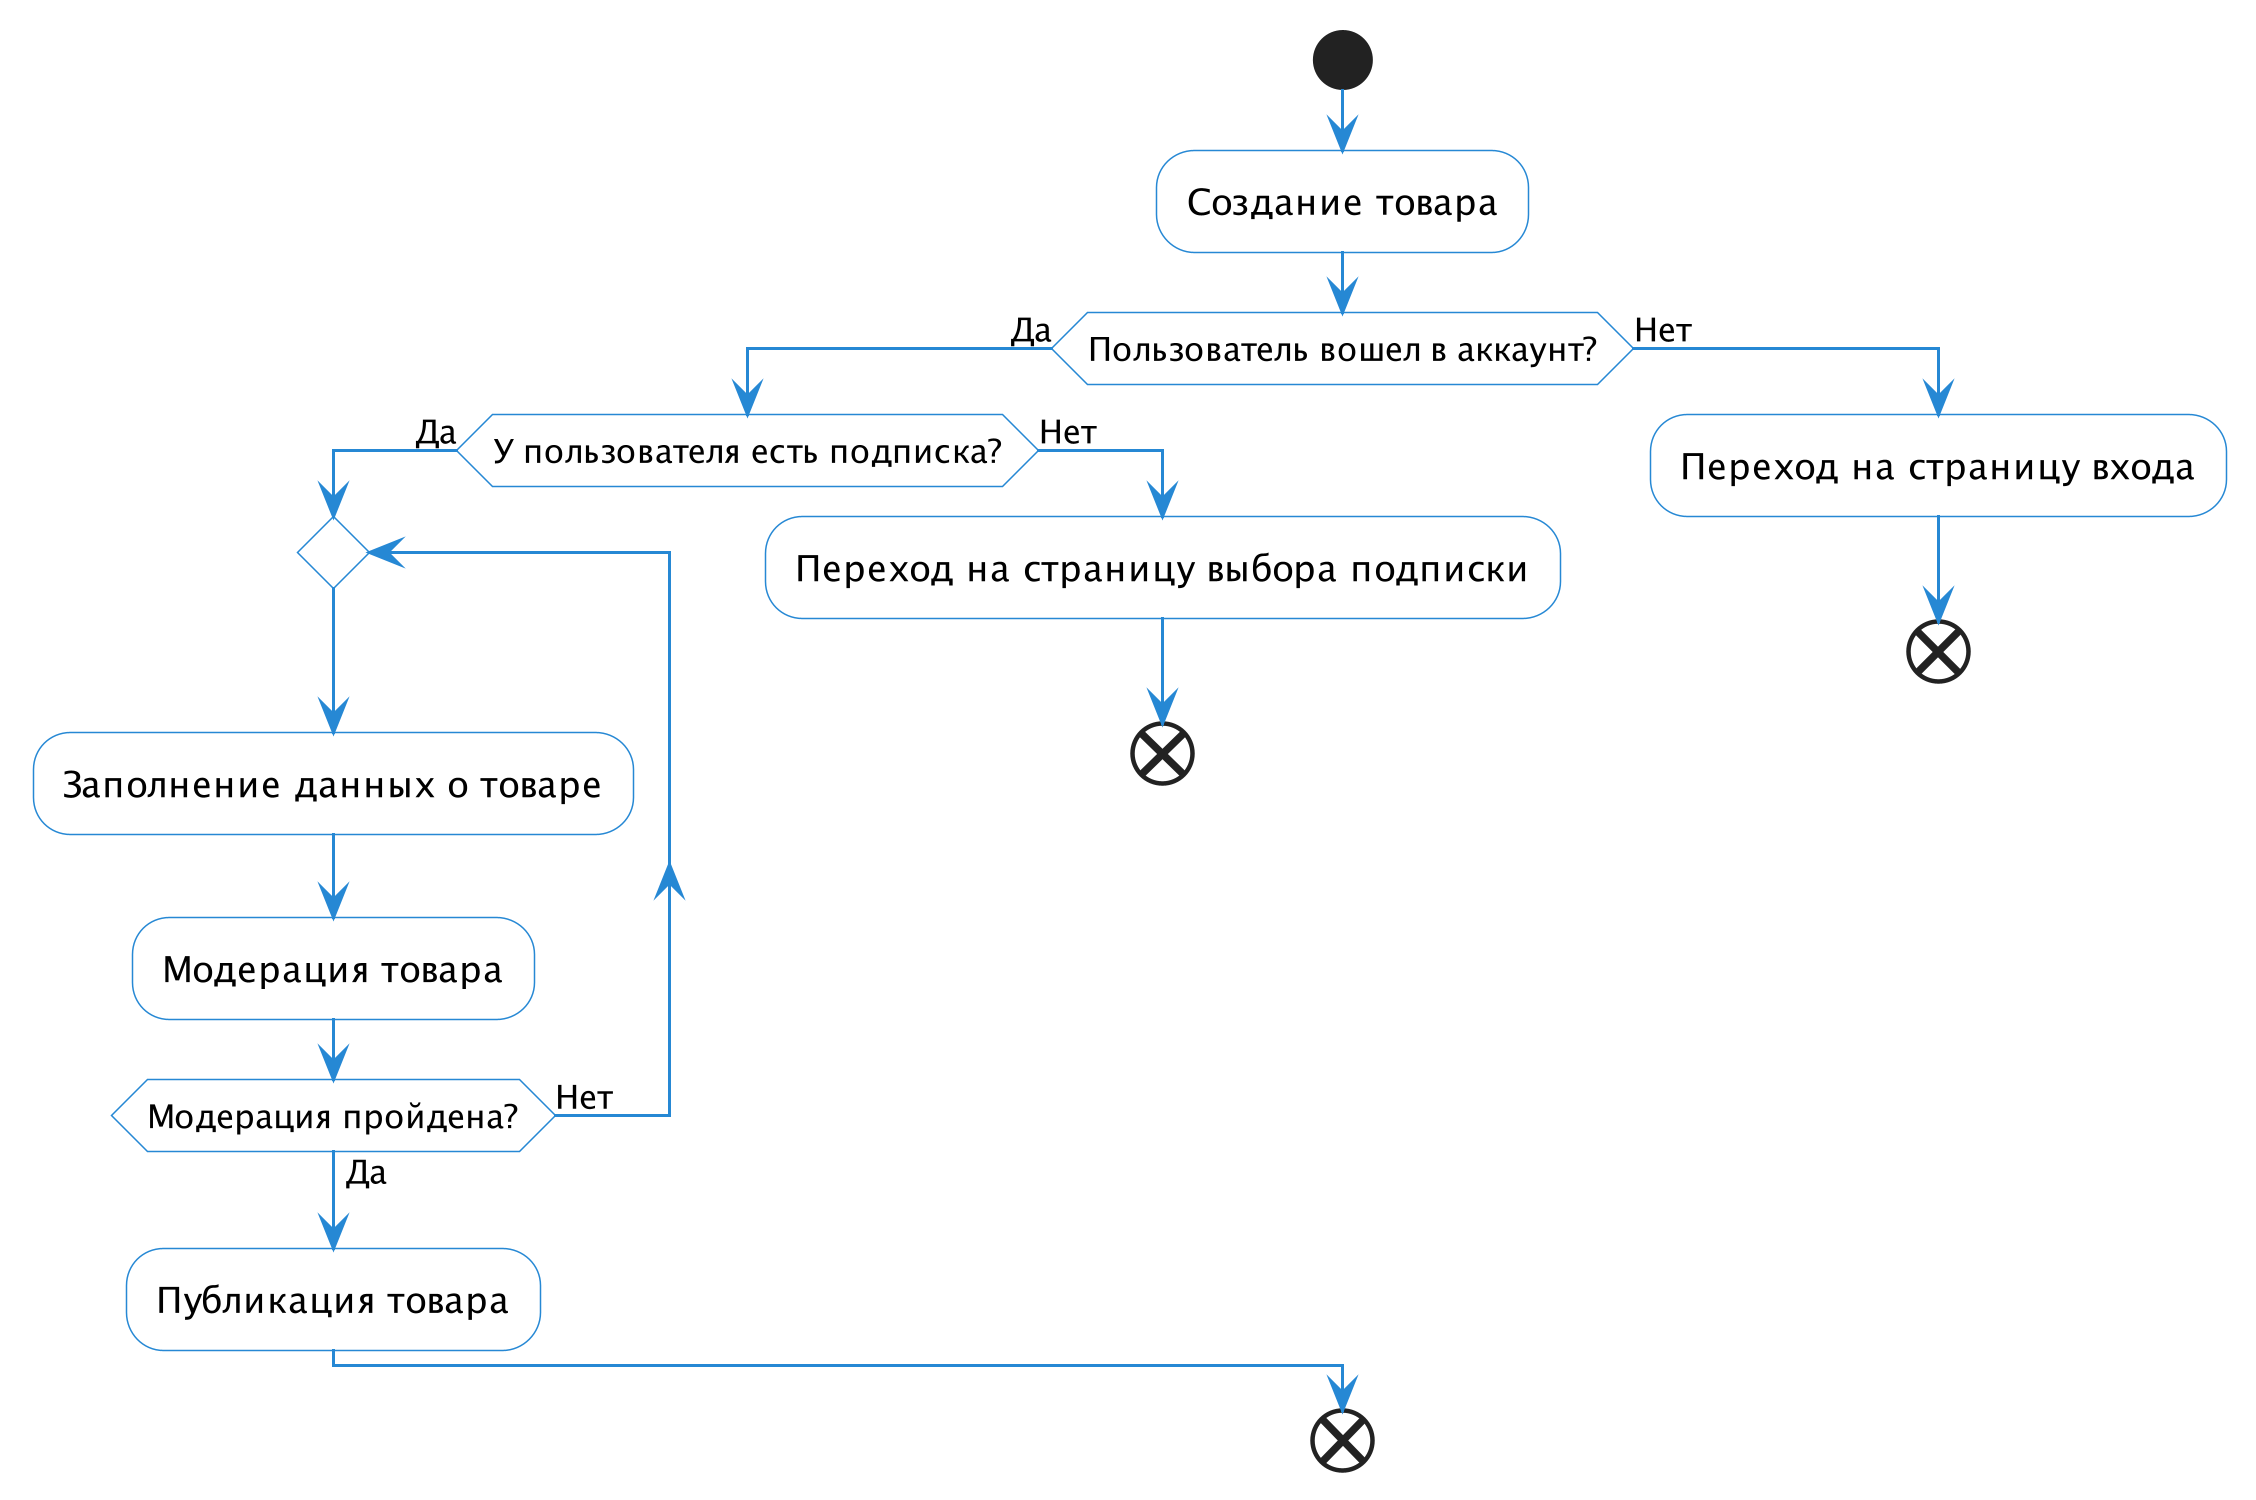
\includegraphics[width=\textwidth]{images/add_item.png}
    \caption{Диаграмма добавления товара на продажу}
\end{figure}

После заполнения формы товар отправляется на модерацию. На модерации товар проверятся по следующим критериям:
\begin{itemize}
    \item \textit{уникальность}: товар не должен быть самым обычным, доступным на каждом углу;
    \item \textit{приемлемое качество}: товар не должен выглядеть как мусор;
    \item \textit{креативность}: товар должен быть интересным, цепляющимся за глаз.
\end{itemize}
Таким образом, модерацию не смогут пройти следующие вещи:
\begin{itemize}
    \item товары широкого потребления;
    \item товары низкого качества;
    \item товары, не содержащие креативной идеи.
\end{itemize}

\subsubsection*{Изменение товара}

После выставления товара на продажу, через некоторое время может появиться необходимость в изменении состояния товара. Так, пользователю доступны следующие состояния товара:
\begin{itemize}
    \item доступен к покупке;
    \item нет в наличии;
    \item продан.
\end{itemize}

\begin{figure}[H]
    \centering
    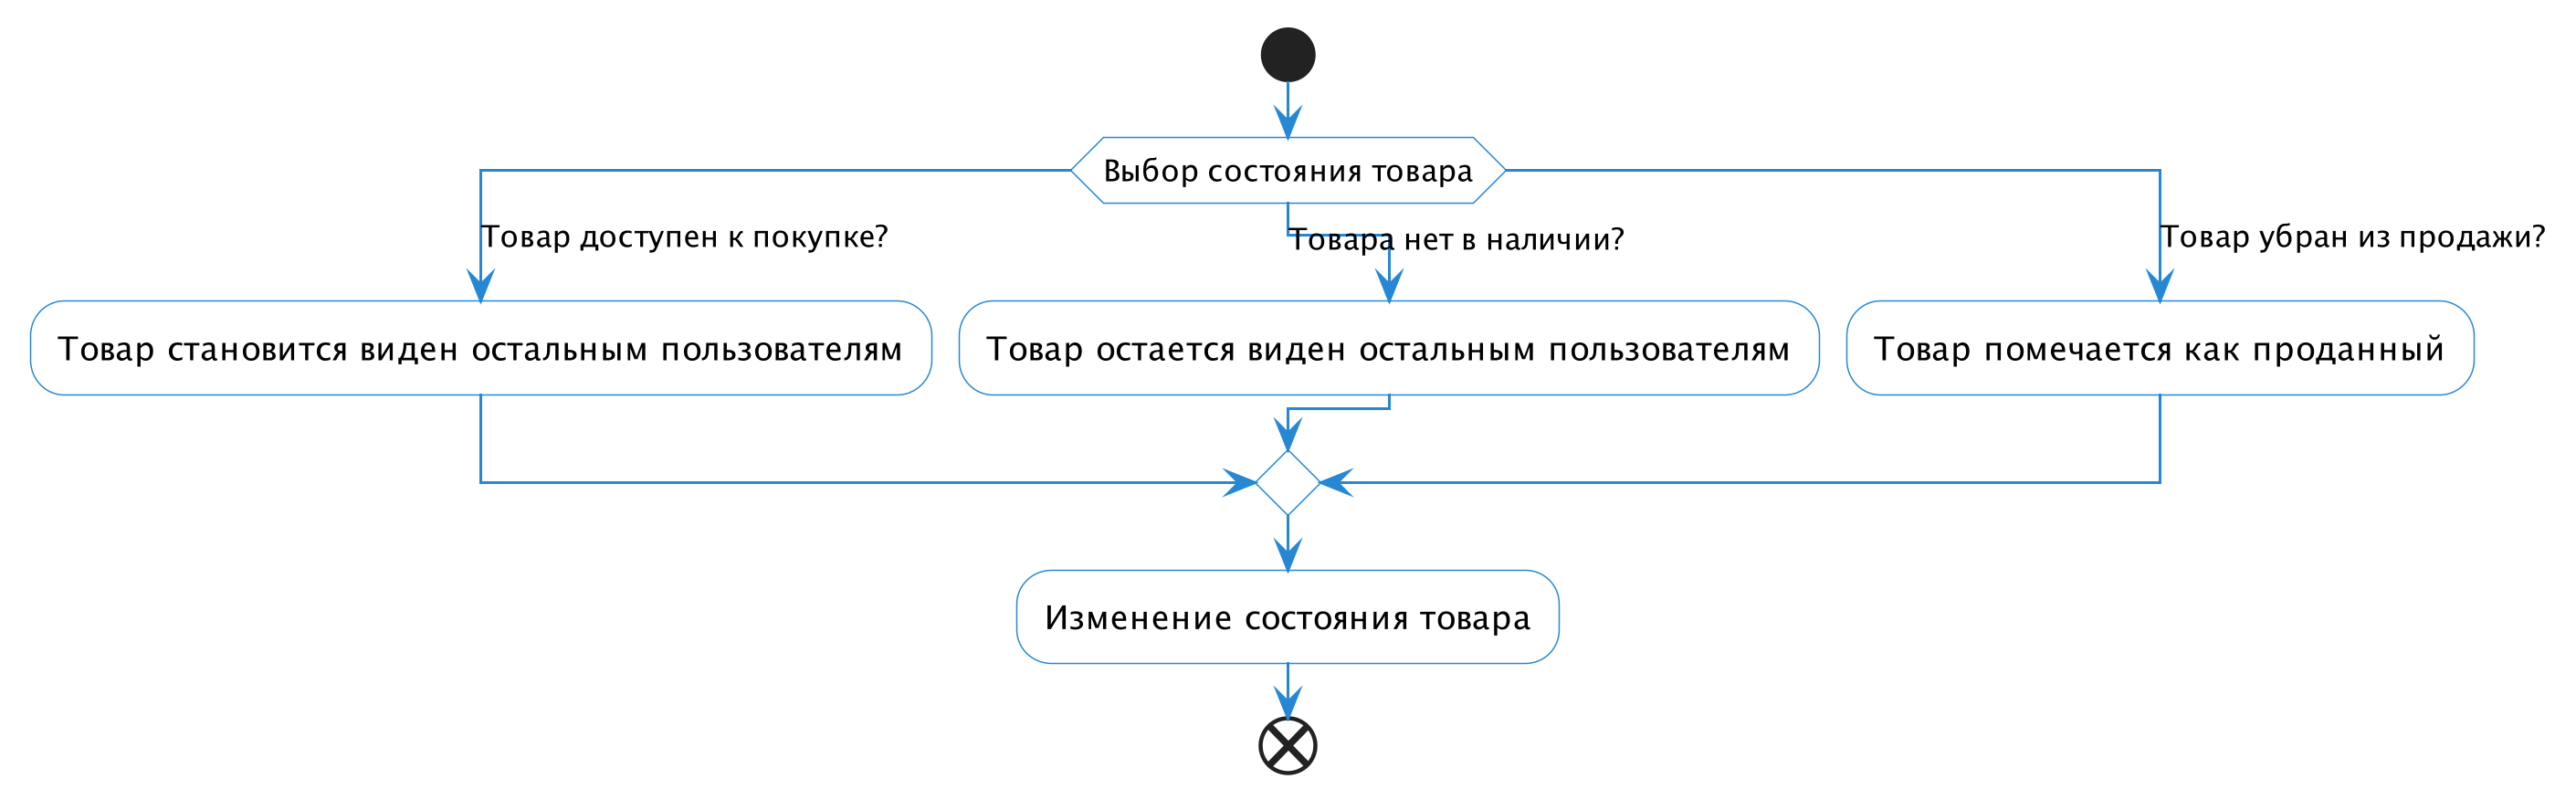
\includegraphics[width=\textwidth]{images/change_item.png}
    \caption{Диаграмма изменения состояния товара}
\end{figure}

В случае, когда товар помечается как доступный к покупке, товар становится виден всем пользователям площадки. При изменении состояния на нет в наличии, товар все еще остается виден пользователям. Однако, если пользователь пометит товар как проданный, то товар будет виден только продавцу. Остальные пользователи площадки не смогут найти его.

\subsubsection*{Добавление товара в избранное}

Чаще всего пользователи делают выбор из нескольких товаров. Поэтому было бы удобно, если можно было бы сохранить понравившиеся товары в отдельный список. Эту функцию реализует система избранных товаров. Пользователю достаточно всего лишь добавить товар в избранное, чтобы не потерять его.

\begin{figure}[H]
    \centering
    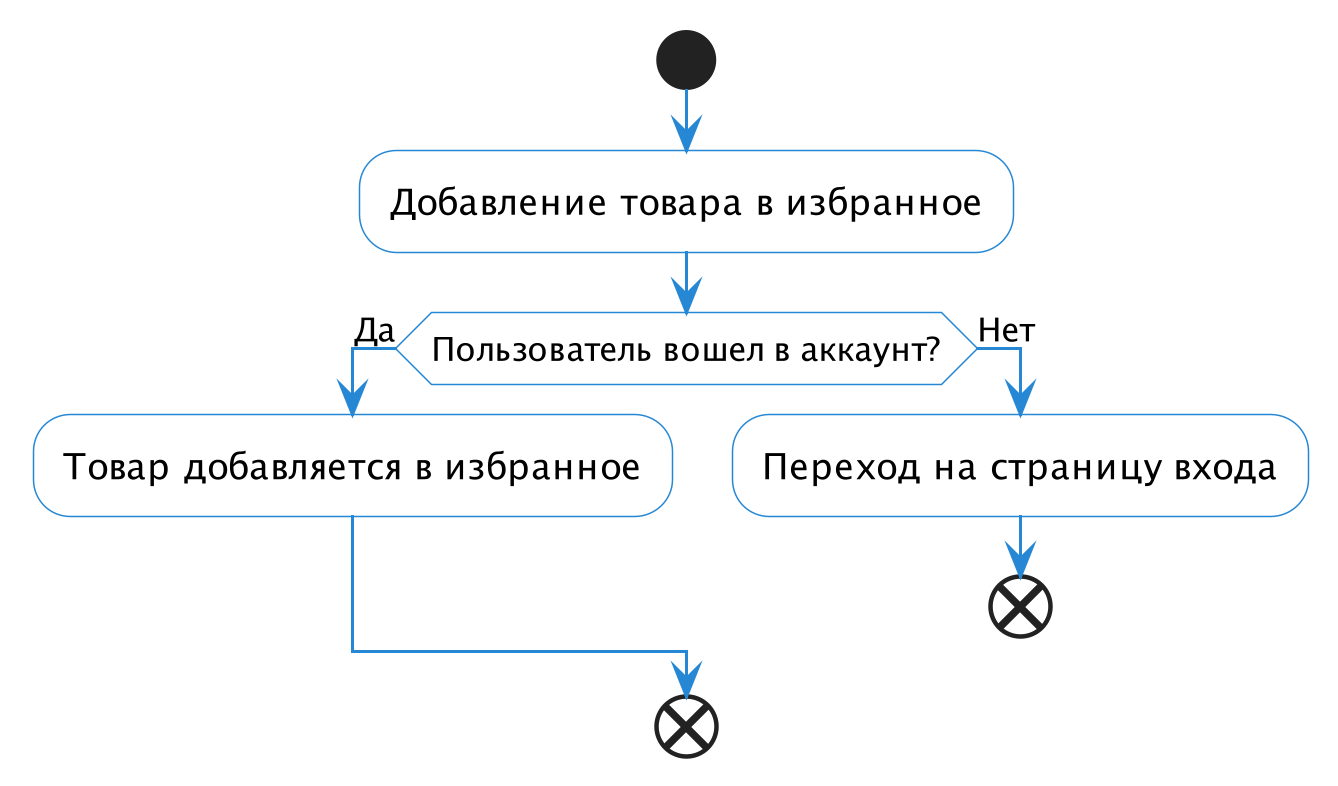
\includegraphics[width=0.7\textwidth]{images/add_to_favourites.png}
    \caption{Диаграмма добавления товара в избранное}
\end{figure}

Единственное условие -- пользователь должен быть авторизован. Мы требуем это, поскольку товары, добавленные в избранное, относятся к конкретному пользователю.

\subsection{Вход в аккаунт}

Теперь рассмотрим процесс входа в аккаунт. Как и всегда, вход в аккаунт делится на две составляющие: регистрацию и авторизацию.

\begin{figure}[H]
    \centering
    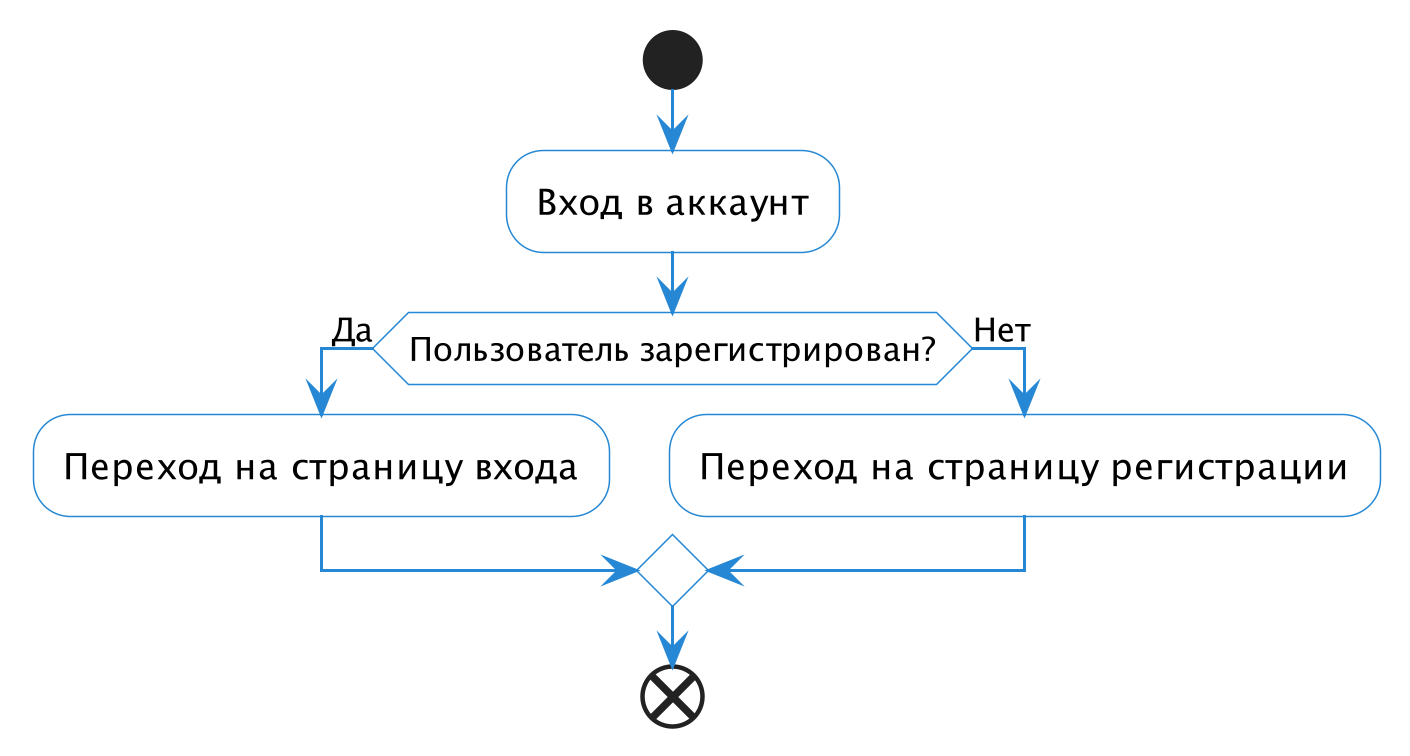
\includegraphics[width=0.7\textwidth]{images/login.png}
    \caption{Диаграмма входа в аккаунт}
\end{figure}

\subsubsection*{Регистрация}

При регистрации проверяется корректность введенных данных. Точнее, проверяются следующие критерии:
\begin{itemize}
    \item пользователя с данной электронной почтой не существует;
    \item пользователя с данным ником не существует;
    \item ник не содержит запрещенных слов;
    \item пароль состоит минимум из 8 символов.
\end{itemize}
После регистрации пользователь попадает на страницу авторизации.

\begin{figure}[H]
    \centering
    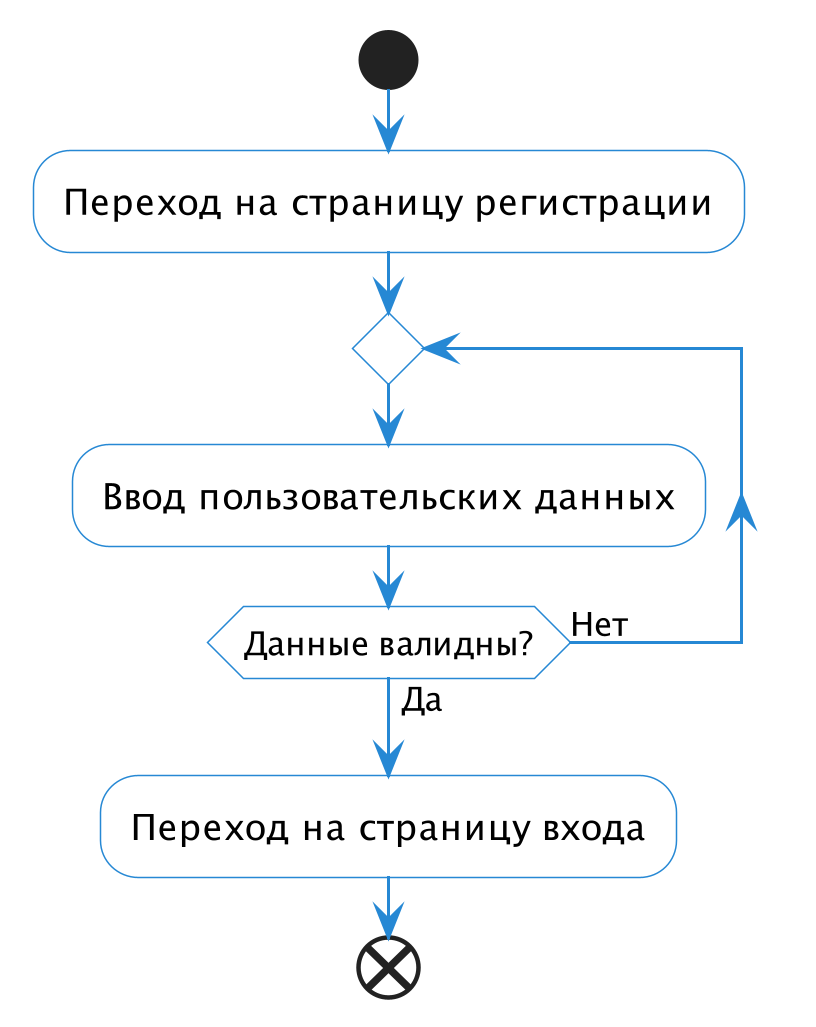
\includegraphics[height=0.4\textheight]{images/register.png}
    \caption{Диаграмма регистрации}
\end{figure}

\subsubsection*{Авторизация}

При авторизации сначала проверяется корректность введенных данных. После этого, проверяется, подтвержден ли текущий аккаунт. Аккаунт подтверждается с помощью перехода по ссылке, которая приходит на электронную почту. Если аккаунт подтвержден, то процесс авторизации завершен. Иначе, пользователь может потребовать выслать новую ссылку для подтверждения аккаунта.

\begin{figure}[H]
    \centering
    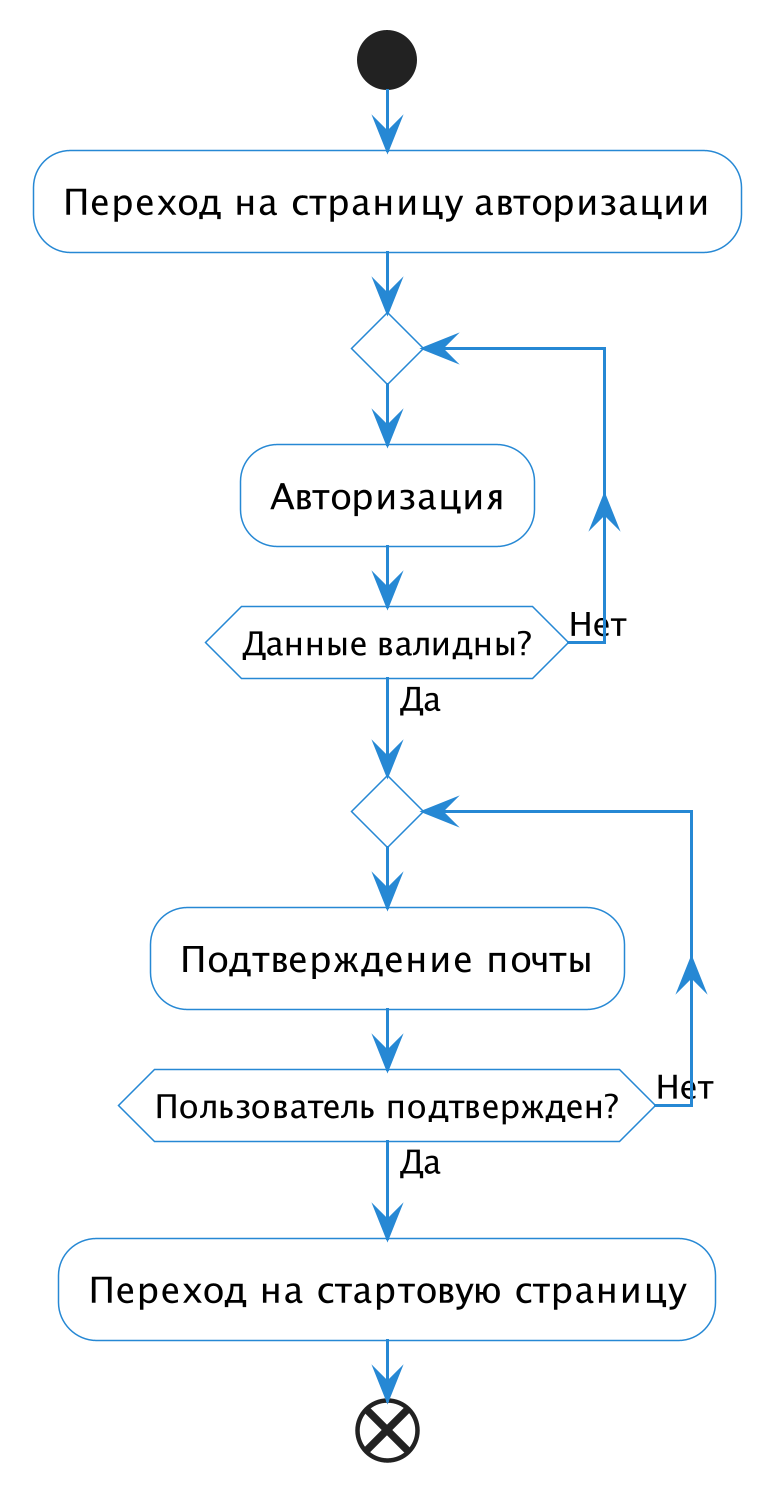
\includegraphics[height=0.5\textheight]{images/auth.png}
    \caption{Диаграмма авторизации}
\end{figure}

\subsection{Приобретение подписки}

Для добавления товара на площадку необходимо выполнить как минимум два условия: быть авторизованным и иметь подписку на своем аккаунте. Рассмотрим процесс приобретения подписки подробнее.

\begin{figure}[H]
    \centering
    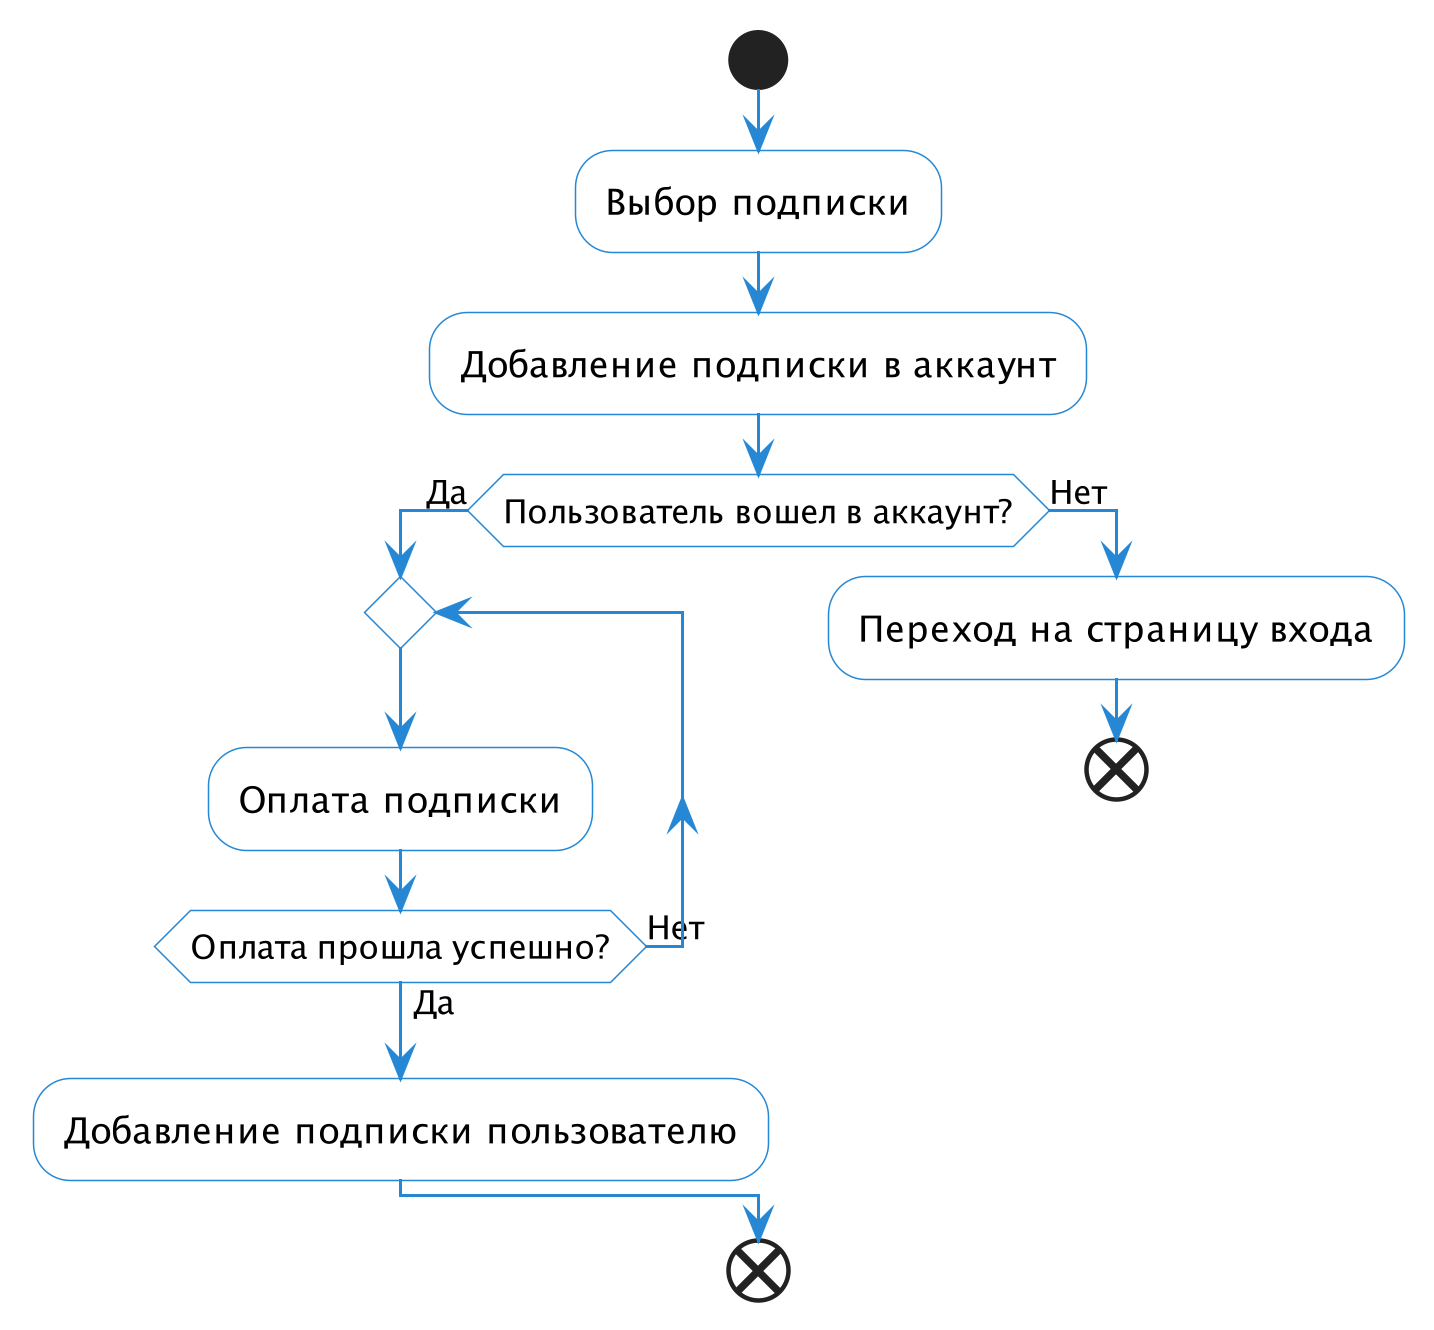
\includegraphics[width=0.65\textwidth]{images/subscription.png}
    \caption{Диаграмма добавления подписки}
\end{figure}

Прежде всего, пользователю необходимо определиться, какую подписку он собирается приобрести. В следующей таблице приведены примерные виды подписки.

\begin{center}
    % \renewcommand{\arraystretch}{1.5}
    \begin{longtable}{|>{\centering\arraybackslash}m{5cm}|>{\centering\arraybackslash}m{5cm}|>{\centering\arraybackslash}m{5.5cm}|}
        \caption{Примеры подписок} \\
        \hline
        \textbf{Название} & \textbf{Длительность} & \textbf{Стоимость} \\
        \hline
        Право имеющий     & 1 месяц               & 300 рублей         \\
        \hline
        Твоя роза         & 3 месяца              & 777 рублей         \\
        \hline
        Замена счастию    & 6 месяцев             & 1337 рублей        \\
        \hline
        Часть той силы    & 12 месяцев            & 2048 рублей        \\
        \hline
    \end{longtable}
\end{center}

После выбора подписки, пользователь должен оплатить ее. В случае успешного завершения оплаты, подписка добавляется на аккаунт пользователя.

\subsection{Добавление отзывов}

Пользователи могут добавлять отзывы на продавцов. В отличии от товаров, отзывы видны сразу после их добавления. Однако отзыв может быть удален, если не он не пройдет модерацию.

\begin{figure}[H]
    \centering
    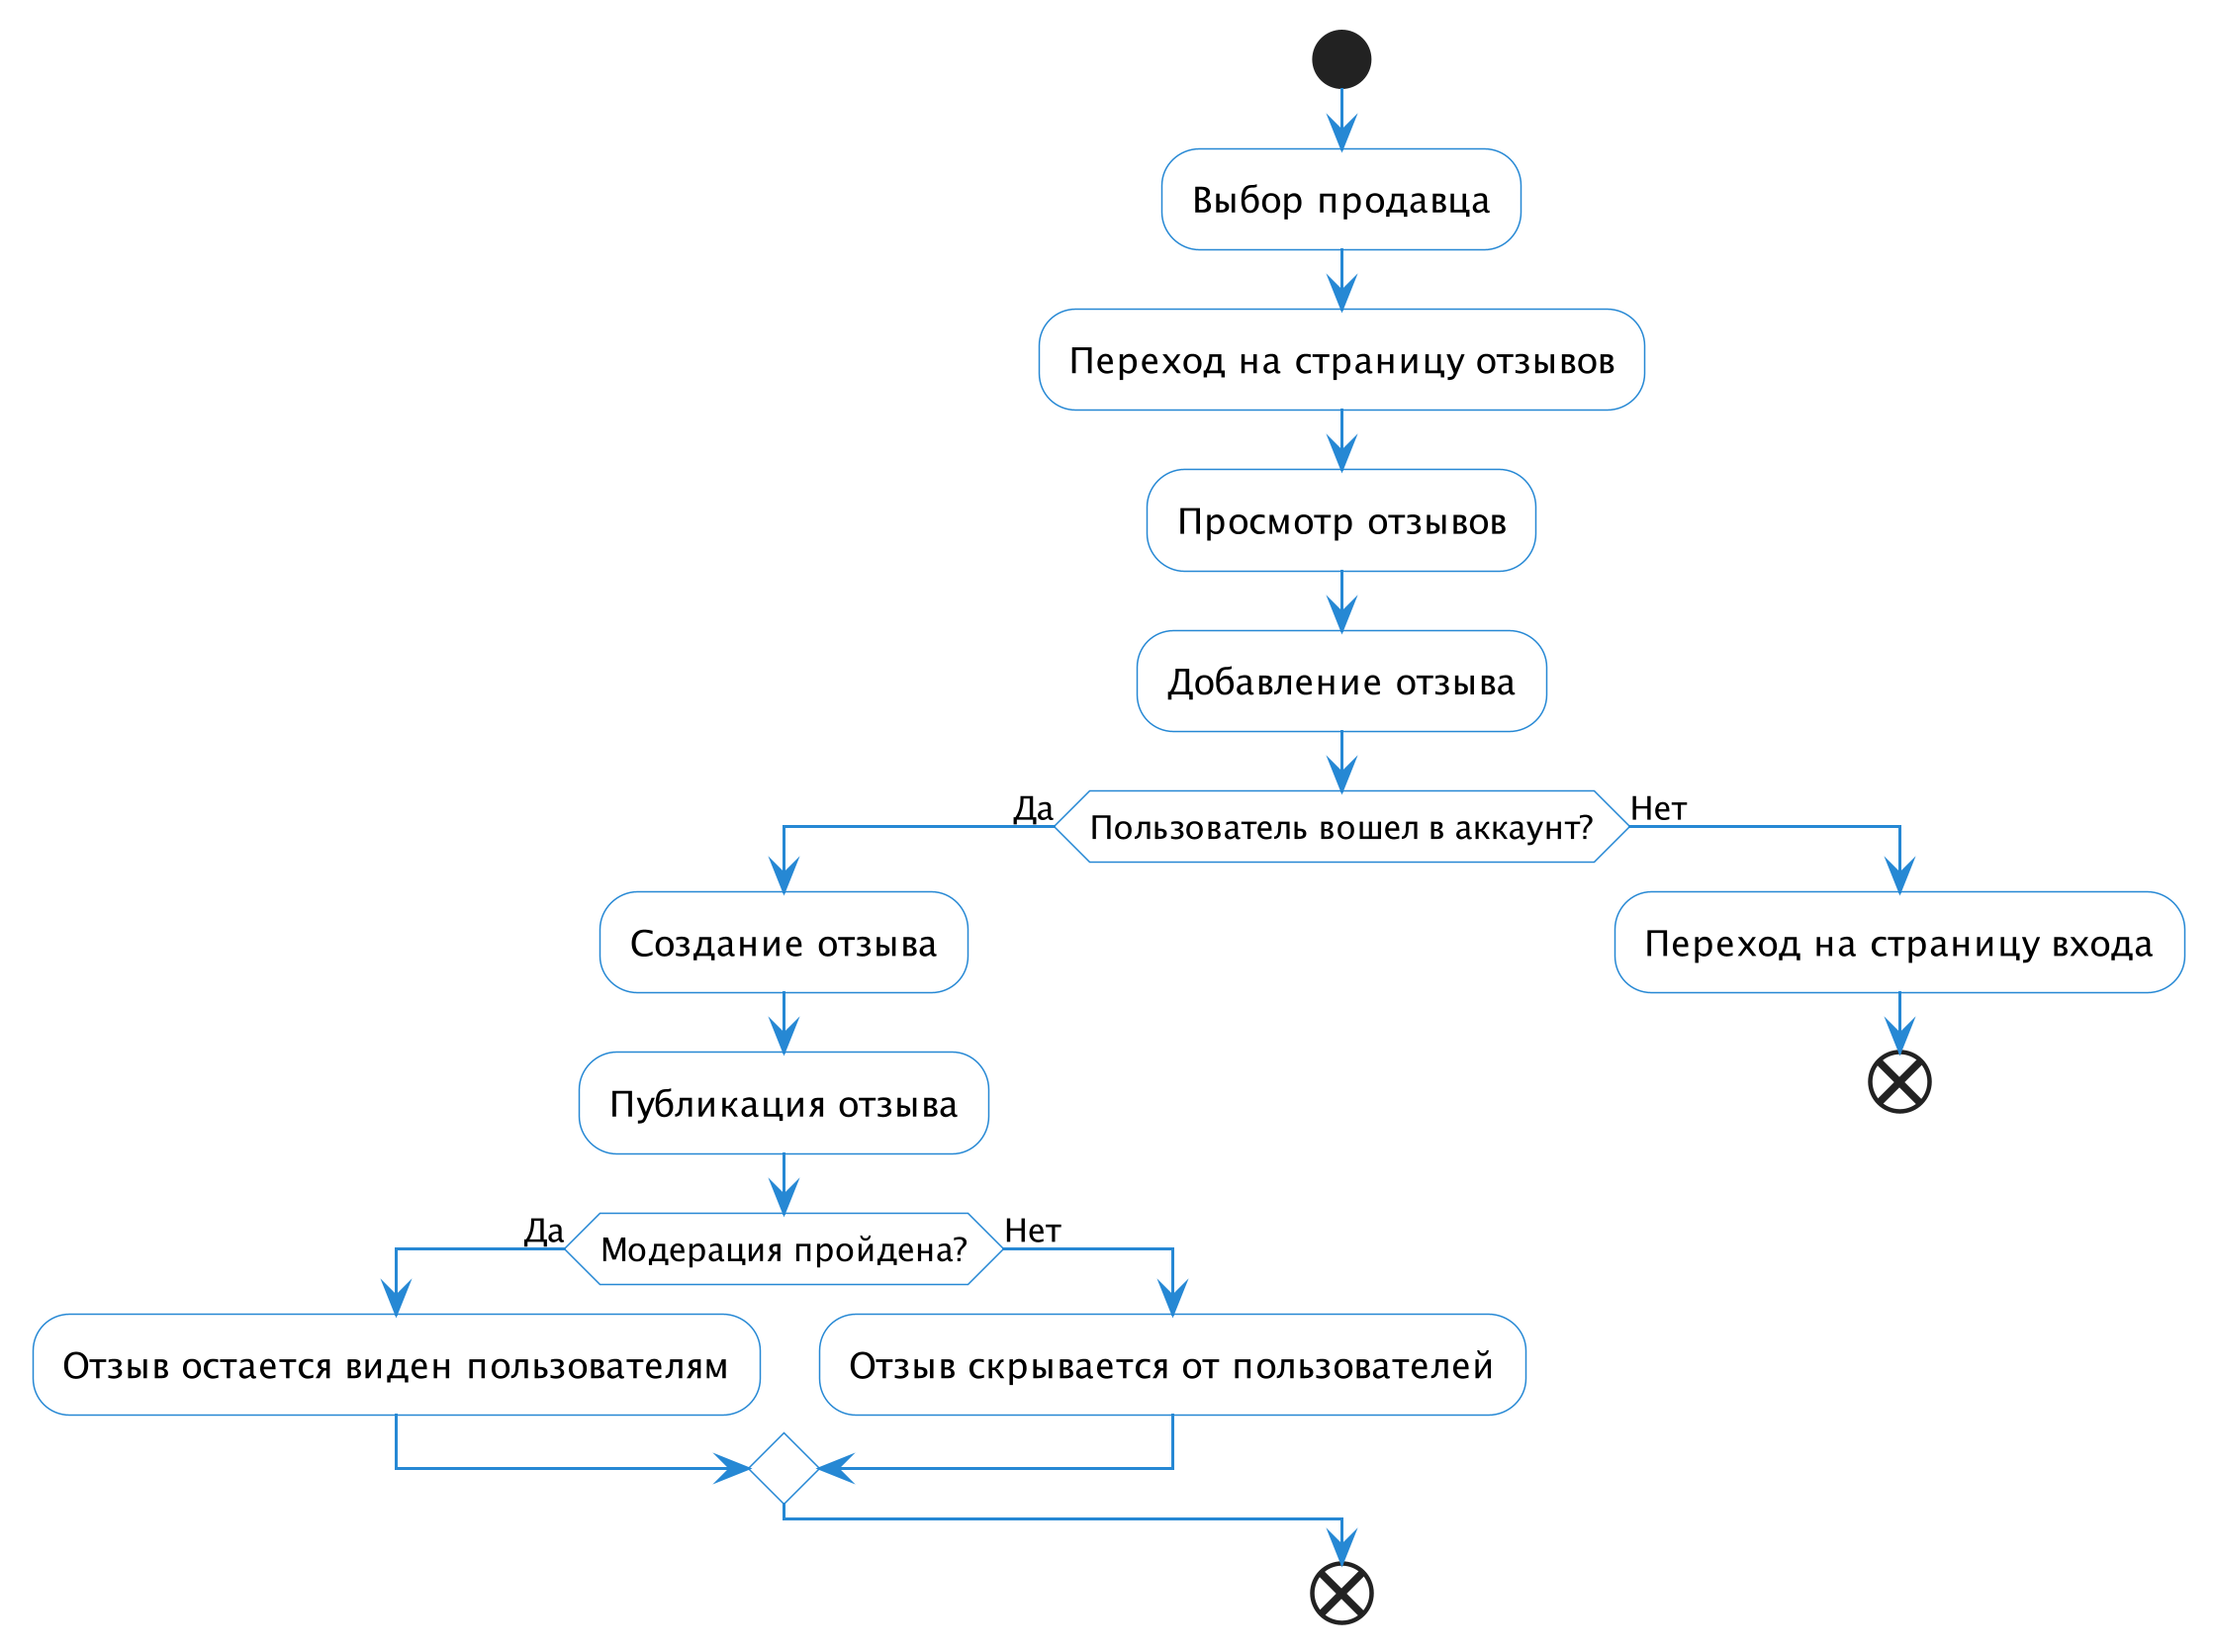
\includegraphics[width=\textwidth]{images/user_feedback.png}
    \caption{Диаграмма добавления отзыва к продавцу}
\end{figure}

% \subsection{Чат с продавцом}

% TODO: добавить изображение


\section{Проектирование базы данных}

На рисунке \ref{fig:db} представлена схема получившейся в ходе разработки базы данных. В этом разделе мы подробно рассмотрим причины тех или иных решений.

\begin{figure}[H]
    \centering
    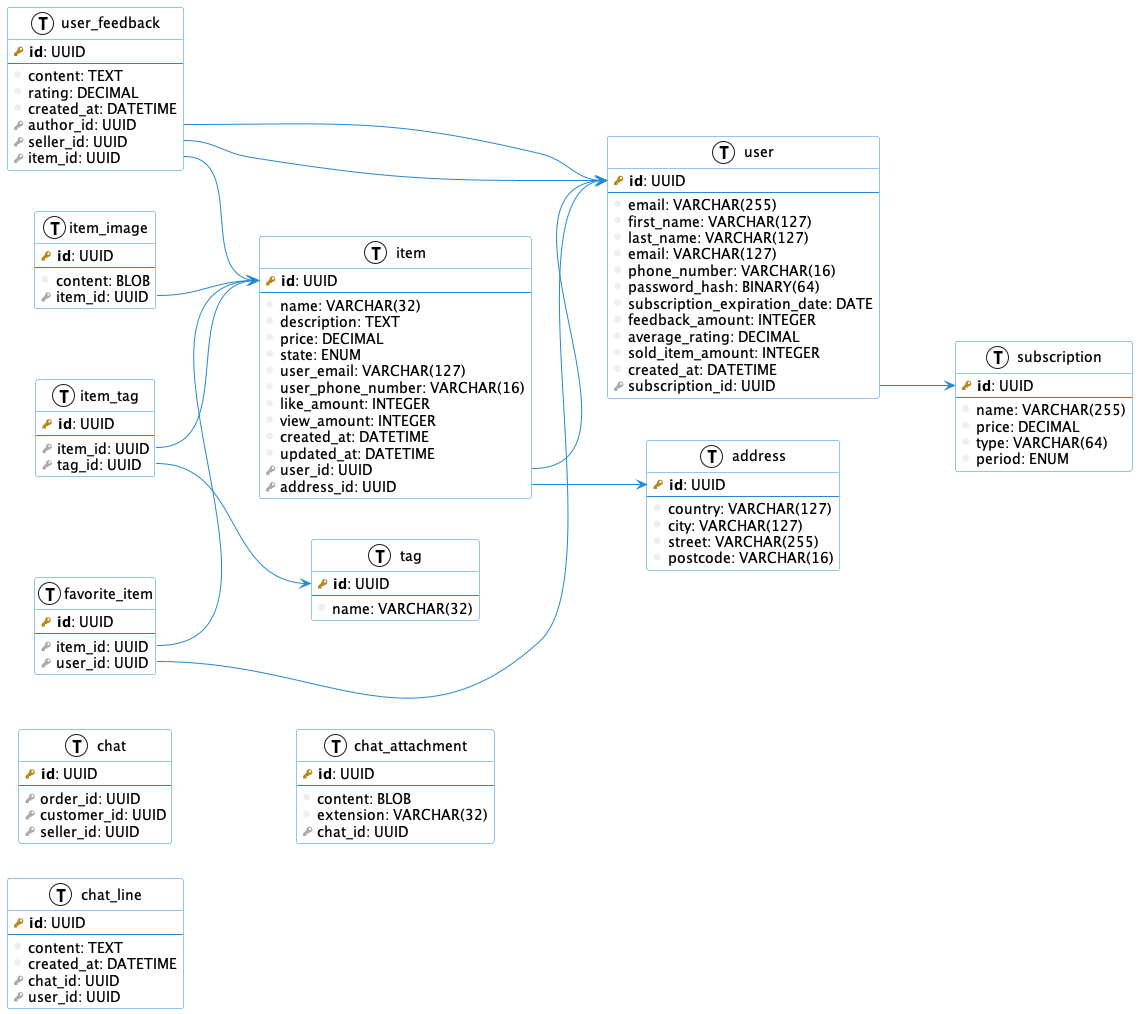
\includegraphics[width=\textwidth]{images/db.png}
    \caption{Диаграмма базы данных}
    \label{fig:db}
\end{figure}

\subsection{Пользователи}

Для начала рассмотрим устройство пользователя в нашей системе. Прежде всего каждый пользователь должен иметь информацию об электронной почте, нике и пароле. Для безопасности пароль будем хранить в захешированном виде. Кроме того, пользователь также может указать информацию о своем имени и фамилии, номере телефона. Поскольку мы предполагаем наличие рейтинговой системы у каждого пользователя, нам также нужно хранить количество отзывов и их среднее значение. Также было решено хранить дату создания аккаунта и количество проданных товаров. Описание получившихся полей этой таблицы представлено в таблице \ref{tab:user}.

\begin{center}
    \begin{longtable}{|c|c|>{\centering\arraybackslash}m{8cm}|}
        \caption{Описание полей таблицы \texttt{user}}
        \label{tab:user}
        \\
        \hline
        \textbf{Название}           & \textbf{Тип}          & \textbf{Описание}                                                                     \\
        \hline
        \texttt{id}                 & \texttt{UUID}         & Идентификатор пользователя. Первичный ключ                                            \\
        \hline
        \texttt{email}              & \texttt{VARCHAR(255)} & Почта пользователя. Обязательное поле                                                 \\
        \hline
        \texttt{username}           & \texttt{VARCHAR(32)}  & Ник пользователя. Обязательное поле                                                   \\
        \hline
        \texttt{first\_name}        & \texttt{VARCHAR(127)} & Имя пользователя                                                                      \\
        \hline
        \texttt{last\_name}         & \texttt{VARCHAR(127)} & Фамилия пользователя                                                                  \\
        \hline
        \texttt{phone\_number}      & \texttt{VARCHAR(16)}  & Телефонный номер пользователя                                                         \\
        \hline
        \texttt{password\_hash}     & \texttt{CHAR(16)}     & Хеш пароль пользователя (SHA-256). Обязательное поле                                  \\
        \hline
        \texttt{feedback\_amount}   & \texttt{INTEGER}      & Количество отзывов у пользователя как продавца. Значение по умолчанию -- \texttt{0}   \\
        \hline
        \texttt{average\_rating}    & \texttt{DECIMAL}      & Средний рейтинг пользователя как продавца. Значение варьируется в интервале от 1 до 5 \\
        \hline
        \texttt{sold\_item\_amount} & \texttt{INTEGER}      & Количество проданных товаров. Значение по умолчанию -- \texttt{0}                     \\
        \hline
        \texttt{created\_at}        & \texttt{DATETIME}     & Дата создания аккаунта                                                                \\
        \hline
    \end{longtable}
\end{center}

Теперь рассмотрим подписочную систему. Прежде всего, у подписки должны быть определены названия, стоимость и время действия. Кроме того, в каждой подписке будем хранить ее тип. Это позволить гибко фильтровать подписки в зависимости от ситуации (например, нам нужно ввести подписки для Нового года, при этом должна быть возможность отображать как старую, так и новую цену). Описание получившихся полей этой таблицы представлено в таблице \ref{tab:subscription}.

\begin{center}
    \begin{longtable}{|c|c|>{\centering\arraybackslash}m{9.8cm}|}
        \caption{Описание полей таблицы \texttt{subscription}}
        \label{tab:subscription}
        \\
        \hline
        \textbf{Название} & \textbf{Тип}          & \textbf{Описание}                                                                                                                               \\
        \hline
        \texttt{id}       & \texttt{UUID}         & Идентификатор подписки. Первичный ключ                                                                                                          \\
        \hline
        \texttt{name}     & \texttt{VARCHAR(255)} & Название подписки. Обязательно поле                                                                                                             \\
        \hline
        \texttt{price}    & \texttt{DECIMAL}      & Стоимость подписки. Обязательное поле                                                                                                           \\
        \hline
        \texttt{type}     & \texttt{VARCHAR(64)}  & Тип подписки. Обязательное поле                                                                                                                 \\
        \hline
        \texttt{period}   & \texttt{ENUM}         & Время действия подписки. В \texttt{ENUM} содержатся следующие значения: \texttt{MONTH}, \texttt{THREE MONTH}, \texttt{HALF YEAR}, \texttt{YEAR} \\
        \hline
    \end{longtable}
\end{center}

Теперь рассмотрим то, как связаны пользователи и подписки. Несмотря на то, что в конкретный момент времени пользователь может иметь только одну активную подписку, нам необходимо хранить не только текущую, но и все предыдущие подписки. Это позволит, при необходимости, ввести систему скидок, которая будет зависеть от количества предыдущих купленных подписок.

Каждая подписка пользователя должна содержать информацию о начале и об окончании срока подписки, а также идентификаторы пользователя и конкретной подписки. Исходя из этого описания, получаем, что мы имеем связь многие ко многим, поскольку один пользователь мог использовать несколько разных подписок за все время, равно как и одна подписка может использоваться у нескольких пользователей сразу. Описание получившихся полей этой таблицы представлено в таблице \ref{tab:user_subscription}.

\begin{center}
    \begin{longtable}{|c|c|>{\centering\arraybackslash}m{9.2cm}|}
        \caption{Описание полей таблицы \texttt{user\_subscription}}
        \label{tab:user_subscription}
        \\
        \hline
        \textbf{Название}         & \textbf{Тип}      & \textbf{Описание}                                                                      \\
        \hline
        \texttt{id}               & \texttt{UUID}     & Идентификатор подписки пользователя. Первичный ключ                                    \\
        \hline
        \texttt{purchased\_at}    & \texttt{DATETIME} & Дата приобретения подписки. Обязательное поле                                          \\
        \hline
        \texttt{expires\_at}      & \texttt{DATETIME} & Дата истечения подписки. Обязательное поле                                             \\
        \hline
        \texttt{user\_id}         & \texttt{UUID}     & Идентификатор пользователя. Внешний ключ на таблицу \texttt{user} поле \texttt{id}     \\
        \hline
        \texttt{subscription\_id} & \texttt{UUID}     & Идентификатор подписки. Внешний ключ на таблицу \texttt{subscription} поле \texttt{id} \\
        \hline
    \end{longtable}
\end{center}

Рассмотрим устройство отзывов на продавцов. Каждый отзыв должен включать в себя свое содержимое, оценку продавца и дату создания отзыва. Кроме этого, поскольку отзывы завязаны на определенный товар, продавца и покупателя, мы должны хранить идентификаторы этих сущностей. Описание получившихся полей этой таблицы представлено в таблице \ref{tab:user_feedback}.

\begin{center}
    \begin{longtable}{|c|c|>{\centering\arraybackslash}m{10.5cm}|}
        \caption{Описание полей таблицы \texttt{user\_feedback}}
        \label{tab:user_feedback}
        \\
        \hline
        \textbf{Название}    & \textbf{Тип}      & \textbf{Описание}                                                                                             \\
        \hline
        \texttt{id}          & \texttt{UUID}     & Идентификатор отзыва. Первичный ключ                                                                          \\
        \hline
        \texttt{content}     & \texttt{TEXT}     & Текстовое содержание отзыва. Обязательное поле                                                                \\
        \hline
        \texttt{rating}      & \texttt{TEXT}     & Оценка, которую поставил пользователь продавцу. Обязательное поле. Значение варьируется в интервале от 1 до 5 \\
        \hline
        \texttt{created\_at} & \texttt{DATETIME} & Дата создания отзыва. Обязательное поле                                                                       \\
        \hline
        \texttt{author\_id}  & \texttt{UUID}     & Идентификатор автора отзыва. Внешний ключ на таблицу \texttt{user} поле \texttt{id}                           \\
        \hline
        \texttt{seller\_id}  & \texttt{UUID}     & Идентификатор продавца. Внешний ключ на таблицу \texttt{user} поле \texttt{id}                                \\
        \hline
        \texttt{item\_id}    & \texttt{UUID}     & Идентификатор товара. Внешний ключ на таблицу \texttt{item} поле \texttt{id}                                  \\
        \hline
    \end{longtable}
\end{center}

Рассмотрим систему добавления товара в избранное. Для реализации этой системы нам необходимо хранить идентификатор пользователя, добавившего товар, и идентификатор самого товара. Из этого следует, что имеем связь многие ко многим, поскольку несколько товаров может быть добавлено в избранное одним пользователем. В то же время один товар может быть добавлен в избранное несколькими пользователями. Описание получившихся полей этой таблицы представлено в таблице \ref{tab:favourite_item}.

\begin{center}
    \begin{longtable}{|c|c|>{\centering\arraybackslash}m{11.9cm}|}
        \caption{Описание полей таблицы \texttt{favourite\_item}}
        \label{tab:favourite_item}
        \\
        \hline
        \textbf{Название} & \textbf{Тип}  & \textbf{Описание}                                                                  \\
        \hline
        \texttt{id}       & \texttt{UUID} & Идентификатор понравившегося товара. Первичный ключ                                \\
        \hline
        \texttt{item\_id} & \texttt{UUID} & Идентификатор товара. Внешний ключ на таблицу \texttt{item} поле \texttt{id}       \\
        \hline
        \texttt{user\_id} & \texttt{UUID} & Идентификатор пользователя. Внешний ключ на таблицу \texttt{user} поле \texttt{id} \\
        \hline
    \end{longtable}
\end{center}

\subsection{Товары}

Рассмотрим устройство товаров. Каждый товар должен включать название, описание и стоимость. Кроме того, он дополнительно может включат в себя информацию о электронной почте и телефонном номере продавца. Также у каждого товара есть состояние (например, товар находится на модерации). Также, поскольку у пользователей есть возможность добавлять товары в избранное, было решено добавить счетчик людей, добавивших в избранное. Чтобы лучше продвигать тот или иной товар, было решено также хранить количество просмотров товара. Кроме того, мы решили добавить дату создания и дату изменения товара. В добавок ко всему вышеперечисленному, нам необходимо хранить идентификатор продавца. Также было решено у каждого объявления хранить адрес, чтобы ранжировать объявления по городам.

Исходя из вышеперечисленной информации, мы получаем связь один ко многим. Все потому, что у товара может быть только один продавец и один адрес. В это же время один и тот же адрес может быть у нескольких товаров, равно как и продавец может предлагать несколько товаров. Описание получившихся полей этой таблицы представлено в таблице \ref{tab:item}.

\begin{center}
    \begin{longtable}{|c|c|>{\centering\arraybackslash}m{7.5cm}|}
        \caption{Описание полей таблицы \texttt{item}}
        \label{tab:item}
        \\
        \hline
        \textbf{Название}            & \textbf{Тип}          & \textbf{Описание}                                                                                                                                                                     \\
        \hline
        \texttt{id}                  & \texttt{UUID}         & Идентификатор товара. Первичный ключ                                                                                                                                                  \\
        \hline
        \texttt{name}                & \texttt{VARCHAR(32)}  & Название товара. Обязательное поле                                                                                                                                                    \\
        \hline
        \texttt{description}         & \texttt{TEXT}         & Описание товара. Обязательное поле                                                                                                                                                    \\
        \hline
        \texttt{price}               & \texttt{DECIMAL}      & Стоимость товара. Обязательное поле                                                                                                                                                   \\
        \hline
        \texttt{state}               & \texttt{ENUM}         & Состояние товара. Обязательное поле. В \texttt{ENUM} содержатся следующие значения: \texttt{ON MODERATION}, \texttt{IN STOCK}, \texttt{OUT OF STOCK}, \texttt{SOLD}, \texttt{REMOVED} \\
        \hline
        \texttt{user\_email}         & \texttt{VARCHAR(127)} & Электронная почта пользователя                                                                                                                                                        \\
        \hline
        \texttt{user\_phone\_number} & \texttt{VARCHAR(16)}  & Телефонный номер пользователя                                                                                                                                                         \\
        \hline
        \texttt{favourite\_amount}   & \texttt{INTEGER}      & Количество пользователей, добавивших товар в избранное. Значение по умолчанию -- \texttt{0}                                                                                           \\
        \hline
        \texttt{view\_amount}        & \texttt{INTEGER}      & Количество просмотров товара. Значение по умолчанию -- \texttt{0}                                                                                                                     \\
        \hline
        \texttt{created\_at}         & \texttt{DATETIME}     & Дата создания товара. Обязательное поле                                                                                                                                               \\
        \hline
        \texttt{updated\_at}         & \texttt{DATETIME}     & Дата изменения товара                                                                                                                                                                 \\
        \hline
        \texttt{seller\_id}          & \texttt{UUID}         & Идентификатор продавца. Внешний ключ на таблицу \texttt{user} поле \texttt{id}                                                                                                        \\
        \hline
        \texttt{address\_id}         & \texttt{UUID}         & Адрес продажи товара. Внешний ключ на таблицу \texttt{address} поле \texttt{id}                                                                                                       \\
        \hline
    \end{longtable}
\end{center}

Рассмотрим систему картинок товара. К каждому товару может быть приложено несколько картинок. Каждая картинка должна включать в себя имя файла, содержимое и расширение. Кроме этого картинка привязана к определенному товару. Исходя из этого получаем связь один ко многим, поскольку картинка может относится только к одному товару. Однако в то же время у одного товара может быть несколько картинок. Описание получившихся полей этой таблицы представлено в таблице \ref{tab:item_image}.

\begin{center}
    \begin{longtable}{|c|c|>{\centering\arraybackslash}m{10.5cm}|}
        \caption{Описание полей таблицы \texttt{item\_image}}
        \label{tab:item_image}
        \\
        \hline
        \textbf{Название}    & \textbf{Тип}      & \textbf{Описание}                                                            \\
        \hline
        \texttt{id}          & \texttt{UUID}     & Идентификатор изображения товара. Первичный ключ                             \\
        \hline
        \texttt{filename}    & \texttt{BLOB}     & Имя файла. Обязательное поле                                                 \\
        \hline
        \texttt{content}     & \texttt{BLOB}     & Двоичные данные файла. Обязательное поле                                     \\
        \hline
        \texttt{created\_at} & \texttt{DATETIME} & Дата создания изображения                                                    \\
        \hline
        \texttt{item\_id}    & \texttt{UUID}     & Идентификатор товара. Внешний ключ на таблицу \texttt{item} поле \texttt{id} \\
        \hline
    \end{longtable}
\end{center}

Рассмотрим систему тегов. Она довольно проста, поскольку тег должен включат в себя только имя. Описание получившихся полей этой таблицы представлено в таблице \ref{tab:tag}.

\begin{center}
    \begin{longtable}{|c|c|>{\centering\arraybackslash}m{10cm}|}
        \caption{Описание полей таблицы \texttt{tag}}
        \label{tab:tag}
        \\
        \hline
        \textbf{Название} & \textbf{Тип}         & \textbf{Описание}                  \\
        \hline
        \texttt{id}       & \texttt{UUID}        & Идентификатор тега. Первичный ключ \\
        \hline
        \texttt{name}     & \texttt{VARCHAR(32)} & Название тега. Обязательное поле   \\
        \hline
    \end{longtable}
\end{center}

Теперь рассмотрим применение тегов с товарами. Для этого необходимо хранить идентификатор товара, к которому прикреплен тег, а также идентификатор самого тега. Значит, мы имеем дело с связью многие ко многим, поскольку один товар может иметь несколько тегов, а один тег может относиться к нескольким товарам. Описание получившихся полей этой таблицы представлено в таблице \ref{tab:item_tag}.

\begin{center}
    \begin{longtable}{|c|c|>{\centering\arraybackslash}m{11.9cm}|}
        \caption{Описание полей таблицы \texttt{item\_tag}}
        \label{tab:item_tag}
        \\
        \hline
        \textbf{Название} & \textbf{Тип}  & \textbf{Описание}                                                            \\
        \hline
        \texttt{id}       & \texttt{UUID} & Идентификатор тега товара. Первичный ключ                                    \\
        \hline
        \texttt{item\_id} & \texttt{UUID} & Идентификатор товара. Внешний ключ на таблицу \texttt{item} поле \texttt{id} \\
        \hline
        \texttt{tag\_id}  & \texttt{UUID} & Идентификатор тега. Внешний ключ на таблицу \texttt{tag} поле \texttt{id}    \\
        \hline
    \end{longtable}
\end{center}

Рассмотрим адрес, используемый в описании товара. Каждый адрес обязательно должен включать в себя информацию о стране, городе и улице. Кроме этой информации, адрес может включать в себя почтовый индекс. Описание получившихся полей этой таблицы представлено в таблице \ref{tab:address}.

\begin{center}
    \begin{longtable}{|c|c|>{\centering\arraybackslash}m{9.9cm}|}
        \caption{Описание полей таблицы \texttt{address}}
        \label{tab:address}
        \\
        \hline
        \textbf{Название} & \textbf{Тип}          & \textbf{Описание}                    \\
        \hline
        \texttt{id}       & \texttt{UUID}         & Идентификатор адреса. Первичный ключ \\
        \hline
        \texttt{country}  & \texttt{VARCHAR(127)} & Название страны. Обязательное поле   \\
        \hline
        \texttt{city}     & \texttt{VARCHAR(127)} & Название города. Обязательное поле   \\
        \hline
        \texttt{street}   & \texttt{VARCHAR(127)} & Название улицы. Обязательное поле    \\
        \hline
        \texttt{postcode} & \texttt{VARCHAR(16)}  & Почтовый индекс                      \\
        \hline
    \end{longtable}
\end{center}

\subsection{Чат между покупателем и продавцом}

Перед покупкой товара у пользователя может появиться потребность пообщаться с продавцом. Например, покупатель захотел разузнать о товаре поподробнее или, например, пользователь готов купить товар. Для этого покупателю необходимо как-нибудь связаться с продавцом. Наша площадка предлагает несколько путей для решения этой проблемы.

Как было показано ранее, у каждого товара обязательно есть описание. Кроме того, к описанию можно добавить электронную почту и телефонный номер продавца. Таким образом, с помощью каких-либо контактных данных в описании товара, электронной почты или телефона покупатель может связаться с продавцом для уточнения своих вопросов.

Однако это не единственный способ связи покупателя с продавцом. Наша площадка предоставляет минимально необходимый функционал для общения покупателей и продавцов. Для каждого товара между покупателем и продавцом создается чат, в котором можно отправлять как текстовые сообщения, так и различные файлы, в том числе и картинки.

Исходя из вышеописанного функционала, можно выделить три сущности: чат, сообщения и вложения. Рассмотрим каждый из них поподробнее.

Начнем с таблицы чатов. Как было сказано ранее, чаты формируются отдельно для покупателя и продавца для каждого товара. Значит, нам нужно хранить идентификаторы покупателя и продавца, а также идентификатор товара.

Таким образом, мы получаем связь один к многим, поскольку конкретный чат может быть только между определенными пользователями. В то же время одни и те же покупатель и продавец могут переписываться на счет разных товаров. При этом, один продавец может иметь чат с несколькими клиентами для одного товара, а клиент может переписываться с несколькими продавцами на счет нескольких товаров сразу. Описание получившихся полей этой таблицы представлено в таблице \ref{tab:chat}.

\begin{center}
    \begin{longtable}{|c|c|>{\centering\arraybackslash}m{11.2cm}|}
        \caption{Описание полей таблицы \texttt{chat}}
        \label{tab:chat}
        \\
        \hline
        \textbf{Название}     & \textbf{Тип}  & \textbf{Описание}                                                                \\
        \hline
        \texttt{id}           & \texttt{UUID} & Идентификатор чата. Первичный ключ                                               \\
        \hline
        \texttt{item\_id}     & \texttt{UUID} & Идентификатор товара. Внешний ключ на таблицу \texttt{item} поле \texttt{id}     \\
        \hline
        \texttt{customer\_id} & \texttt{UUID} & Идентификатор покупателя. Внешний ключ на таблицу \texttt{user} поле \texttt{id} \\
        \hline
        \texttt{seller\_id}   & \texttt{UUID} & Идентификатор продавца. Внешний ключ на таблицу \texttt{user} поле \texttt{id}   \\
        \hline
    \end{longtable}
\end{center}

Теперь рассмотрим таблицу, отвечающую за хранение конкретного сообщения. Прежде всего каждое сообщение отправляется определенным пользователем, поэтому нам необходимо хранить идентификатор автора сообщения. Кроме того, каждое сообщение привязано к какому-то чату, значит, мы также должны хранить идентификатор чата. Кроме идентификаторов, также необходимо хранить содержимое сообщение и дату создания сообщения.

Исходя из описания, мы получаем связь один ко многим, поскольку определенное сообщение может быть отправлено только одним пользователем в определенном чате. В то же время, пользователь может отправлять несколько сообщений в разных чатах. Описание получившихся полей этой таблицы представлено в таблице \ref{tab:chat_message}.

\begin{center}
    \begin{longtable}{|c|c|>{\centering\arraybackslash}m{10.6cm}|}
        \caption{Описание полей таблицы \texttt{chat\_message}}
        \label{tab:chat_message}
        \\
        \hline
        \textbf{Название}    & \textbf{Тип}      & \textbf{Описание}                                                                      \\
        \hline
        \texttt{id}          & \texttt{UUID}     & Идентификатор сообщения. Первичный ключ                                                \\
        \hline
        \texttt{content}     & \texttt{TEXT}     & Содержание сообщения. Обязательное поле                                                \\
        \hline
        \texttt{created\_at} & \texttt{DATETIME} & Дата создания сообщения. Обязательное поле                                             \\
        \hline
        \texttt{chat\_id}    & \texttt{UUID}     & Идентификатор чата. Внешний ключ на таблицу \texttt{chat} поле \texttt{id}             \\
        \hline
        \texttt{user\_id}    & \texttt{UUID}     & Идентификатор автора сообщения. Внешний ключ на таблицу \texttt{user} поле \texttt{id} \\
        \hline
    \end{longtable}
\end{center}

Рассмотрим таблицу, которая будет хранить в себе содержимое вложения. В первую очередь нам необходимо хранить идентификатор сообщения, к которому относится это вложение. Кроме него, мы также будем хранить имя приложенного файла, его содержимое и расширение этого файла. Также будем хранить дату создания этого вложения.

В этот раз мы также получили связь один ко многим, потому что одно сообщение может включать в себя несколько вложений, однако одно и то же вложение может относиться только к одному сообщению. Описание получившихся полей этой таблицы представлено в таблице \ref{tab:chat_attachment}.

\begin{center}
    \begin{longtable}{|c|c|>{\centering\arraybackslash}m{8.2cm}|}
        \caption{Описание полей таблицы \texttt{chat\_attachment}}
        \label{tab:chat_attachment}
        \\
        \hline
        \textbf{Название}          & \textbf{Тип}          & \textbf{Описание}                                                                        \\
        \hline
        \texttt{id}                & \texttt{UUID}         & Идентификатор вложения. Первичный ключ                                                   \\
        \hline
        \texttt{filename}          & \texttt{VARCHAR(255)} & Имя файла. Обязательное поле                                                             \\
        \hline
        \texttt{content}           & \texttt{BLOB}         & Двоичные данные файла. Обязательное поле                                                 \\
        \hline
        \texttt{extension}         & \texttt{VARCHAR(32)}  & Расширение файла. Обязательное поле                                                      \\
        \hline
        \texttt{created\_at}       & \texttt{DATETIME}     & Дата загрузки файла. Обязательное поле                                                   \\
        \hline
        \texttt{chat\_message\_id} & \texttt{UUID}         & Идентификатор сообщения. Внешний ключ на таблицу \texttt{chat\_message} поле \texttt{id} \\
        \hline
    \end{longtable}
\end{center}

\section{Выводы}

В результате выполнения лабораторной работы удалось спроектировать базу данных для интернет площадки для креативных людей. В процессе выполнения работы были выполнены все поставленные задачи.

Однако во время выполнения возникли некоторые сложности. В первую очередь, было очень сложно сбалансировать систему таким образом, чтобы пользователь чувствовал себя наравне с другими пользователями. При этом, проект нужно каким-то образом монетизировать. В качестве решения этой проблемы была выбрана подписочная система.

Еще одной сложностью стала проблема проектирования. Необходимо было спроектировать систему так, чтобы база данных была готова как к расширению, так и к более серьезным нагрузкам.

В итоге все проявившиеся проблемы удалось решить, как с точки зрения концепта, так и с точки зрения архитектуры базы данных.

\end{document}
